\chapter{Personalization and Recommendation}
\label{ch:recommendation}

\section{Overview and Two Ranking Systems}
\label{sec:rec-overview}

AI Compass contains two ranking mechanisms that must be kept conceptually separate. The first, and the subject of most of this chapter, is the \emph{personalized feed ranking} (\texttt{app/services/ranking\_service.py}'s \texttt{RankingService}), which drives a logged-in user's Home feed and digest email: given a content pool and a specific user, it produces a per-user ordered list with a human-readable explanation for every item. The module declares \texttt{RANKER\_VERSION = "v1-deterministic"}, and its own comment calls it ``a documented, heuristic v1, NOT tuned'': fully deterministic (identical inputs always produce identical scores), but its weights, multipliers, and diversification parameter were set by engineering judgement rather than fit to data.

The second mechanism is a considerably simpler, entirely \emph{non-personalized} formula powering the public Home feed shown to a signed-out visitor (\texttt{web/apps/news/feed\_ranking.py}). It shares no code, weights, or behavioral inputs with the personalized ranker; Section~\ref{sec:rec-public-feed} treats it separately so the two are never conflated.

The personalized ranker is a three-stage pipeline followed in order below: \emph{candidate generation} (Section~\ref{sec:rec-candidates}) assembles a bounded eligible pool; \emph{scoring} (Section~\ref{sec:rec-score}) assigns each candidate a deterministic score from five weighted signals adjusted by bounded multipliers; and \emph{selection} (Section~\ref{sec:rec-mmr}) greedily builds the final list under a diversity objective plus a reserved exploration slice. Every selected item receives a templated, non-generative explanation (Section~\ref{sec:rec-explanations}). Section~\ref{sec:rec-pipeline} recaps the pipeline as a figure; Sections~\ref{sec:rec-deferred}--\ref{sec:rec-limitations} close with what was deliberately left out of scope and what was not.

\section{Behavioral Signal Aggregation}
\label{sec:rec-signals}

Personalization begins with raw behavioral events. AI Compass records six event types against a user and a content item: \texttt{impression}, \texttt{click}, \texttt{save}, \texttt{hide}, \texttt{dwell} (time spent on an item), and \texttt{digest\_click} (a link opened from a digest email). These events are the only input to two nightly-recomputed structures that the personalized ranker later reads: \texttt{UserAffinity}, a per-user set of decaying weights along three dimensions (\texttt{topic}, \texttt{source}, and \texttt{entity}), and \texttt{UserProfileVector}, a single per-user embedding summarizing the content the user has actually engaged with.

Both structures are built from the same nightly job over a rolling 90-day window of events, and both apply the same exponential recency decay, with a half-life of 14 days, to each event before it contributes to the aggregate:

\begin{equation}
\text{weight}(u, d) = \sum_{e \,\in\, E_u(d)} w(e) \cdot e^{-\lambda \cdot \text{age\_days}(e)}, \qquad \lambda = \frac{\ln 2}{14}
\label{eq:affinity-decay}
\end{equation}

\noindent where $E_u(d)$ is the set of events belonging to user $u$ associated with dimension value $d$ (a topic, source, or entity), $w(e)$ is a fixed weight per event type, and $\text{age\_days}(e)$ is the event's age at aggregation time. With $\lambda = \ln 2/14$, an event's contribution is exactly halved every 14 days without reinforcement, so recent behavior dominates while older behavior fades smoothly rather than being discarded at a fixed cutoff.

The event-type weights $w(e)$ are asymmetric by design: \texttt{impression} $= 0.1$, \texttt{click} $= 1.0$, \texttt{save} $= 3.0$, \texttt{digest\_click} $= 1.5$: a save counts as a substantially stronger interest signal than a click, and a click stronger than a mere impression. \texttt{hide} is deliberately \emph{negative}, $-2.0$: an explicit rejection actively pulls the corresponding affinity downward rather than merely failing to reinforce it. \texttt{dwell} is folded in as an additional graded engagement signal.

\texttt{UserProfileVector} is built from the same 90-day window, but over a narrower subset of events: only \texttt{click}, \texttt{save}, \texttt{dwell}, and \texttt{digest\_click} contribute, while \texttt{impression} and \texttt{hide} are excluded. It is a decayed, weighted mean of the embeddings behind those qualifying events, L2-normalized before storage so it can be compared to candidate embeddings by cosine similarity. The job wholesale-recomputes this vector nightly rather than updating it incrementally, so it always reflects the exact current 90-day window with no accumulated online-update drift.

\section{Candidate Generation}
\label{sec:rec-candidates}

Before any item can be scored for a given user, it must first survive an \emph{eligibility filter} and then be admitted into a bounded \emph{candidate pool} through one of three routes. The eligibility filter is applied first and is a hard gate, not a scoring adjustment: an item is dropped outright if its source has been excluded by the user, if its content category has been excluded by the user, or if it belongs to a source whose visibility is \texttt{user}-restricted and the requesting user is not subscribed to it. Only items that survive this filter are eligible to enter the candidate pool through any of the three legs described below.

The three legs are a union, not alternatives: an item qualifying through more than one leg is still scored once. \emph{Leg A (recency)} contributes the newest 300 eligible items by \texttt{published\_at}, giving every pool a baseline of current content. \emph{Leg B (similarity)} performs a pgvector nearest-neighbor search against the user's \texttt{UserProfileVector} (Section~\ref{sec:rec-signals}), returning up to 150 closest items by embedding; with no profile vector yet (cold start), it falls back to items whose topic overlaps the user's onboarding interests. \emph{Leg C (follows)} guaranteedly admits any item matching a followed topic, entity, source, or followed person's footprint (blog, GitHub, or YouTube channel); it is the only leg that bypasses recency and similarity entirely, so an old item from a followed source is still admitted. The union is capped at 300 candidates before scoring.

Leg C is also the one place where the platform's Free/Pro entitlement distinction touches candidate generation, and it is worth stating precisely how: a Free-plan user is limited to \texttt{FREE\_FOLLOW\_LIMIT} = 20 follow relationships, while a Pro-plan user may hold an unlimited number. This limit bounds how many items \emph{can possibly} enter through Leg C for a Free user; it does not alter the scoring formula, the multipliers, or the diversification step in any way for either plan. There is no Free/Pro branch anywhere inside the scoring logic itself; the only interaction between entitlements and ranking is this indirect, upstream effect on how much material a Free user's follows can guarantee into the candidate pool before scoring ever begins.

Algorithm~\ref{alg:candidates} summarizes the process.

\begin{algorithm}[htbp]
\DontPrintSemicolon
\KwInput{user $u$, eligible content pool $P$ (after the eligibility filter)}
\KwOutput{candidate pool $C$, $|C| \le 300$}
$A \leftarrow$ top 300 items of $P$ ordered by $\text{published\_at}$ descending\tcp*{Leg A: recency}
\If{$u$ has a stored \texttt{UserProfileVector} $v_u$}{
  $B \leftarrow$ top 150 items of $P$ by cosine similarity to $v_u$ (pgvector ANN search)\tcp*{Leg B: similarity}
}
\Else{
  $B \leftarrow \{\, p \in P : \text{topic}(p) \in \text{onboarding\_interests}(u) \,\}$\tcp*{Leg B cold-start fallback}
}
$F \leftarrow \{\, p \in P : p \text{ matches a followed topic, entity, source, or followed-person footprint} \,\}$\tcp*{Leg C: follows}
$C \leftarrow A \cup B \cup F$, retaining every item in $F$ and truncating $A \cup B$ as needed to cap $|C|$ at 300\;
\Return{$C$}
\caption{Candidate generation (three-leg union)}
\label{alg:candidates}
\end{algorithm}

Figure~\ref{fig:screenshot-preferences} shows the standalone Preferences page that supplies the \texttt{onboarding\_interests}(u) set used by Leg B's cold-start fallback above: a user who has not yet accumulated enough behavioral history for a \texttt{UserProfileVector} instead has their candidate pool shaped directly by the topic chips selected here.

\begin{figure}[htbp]
\centering
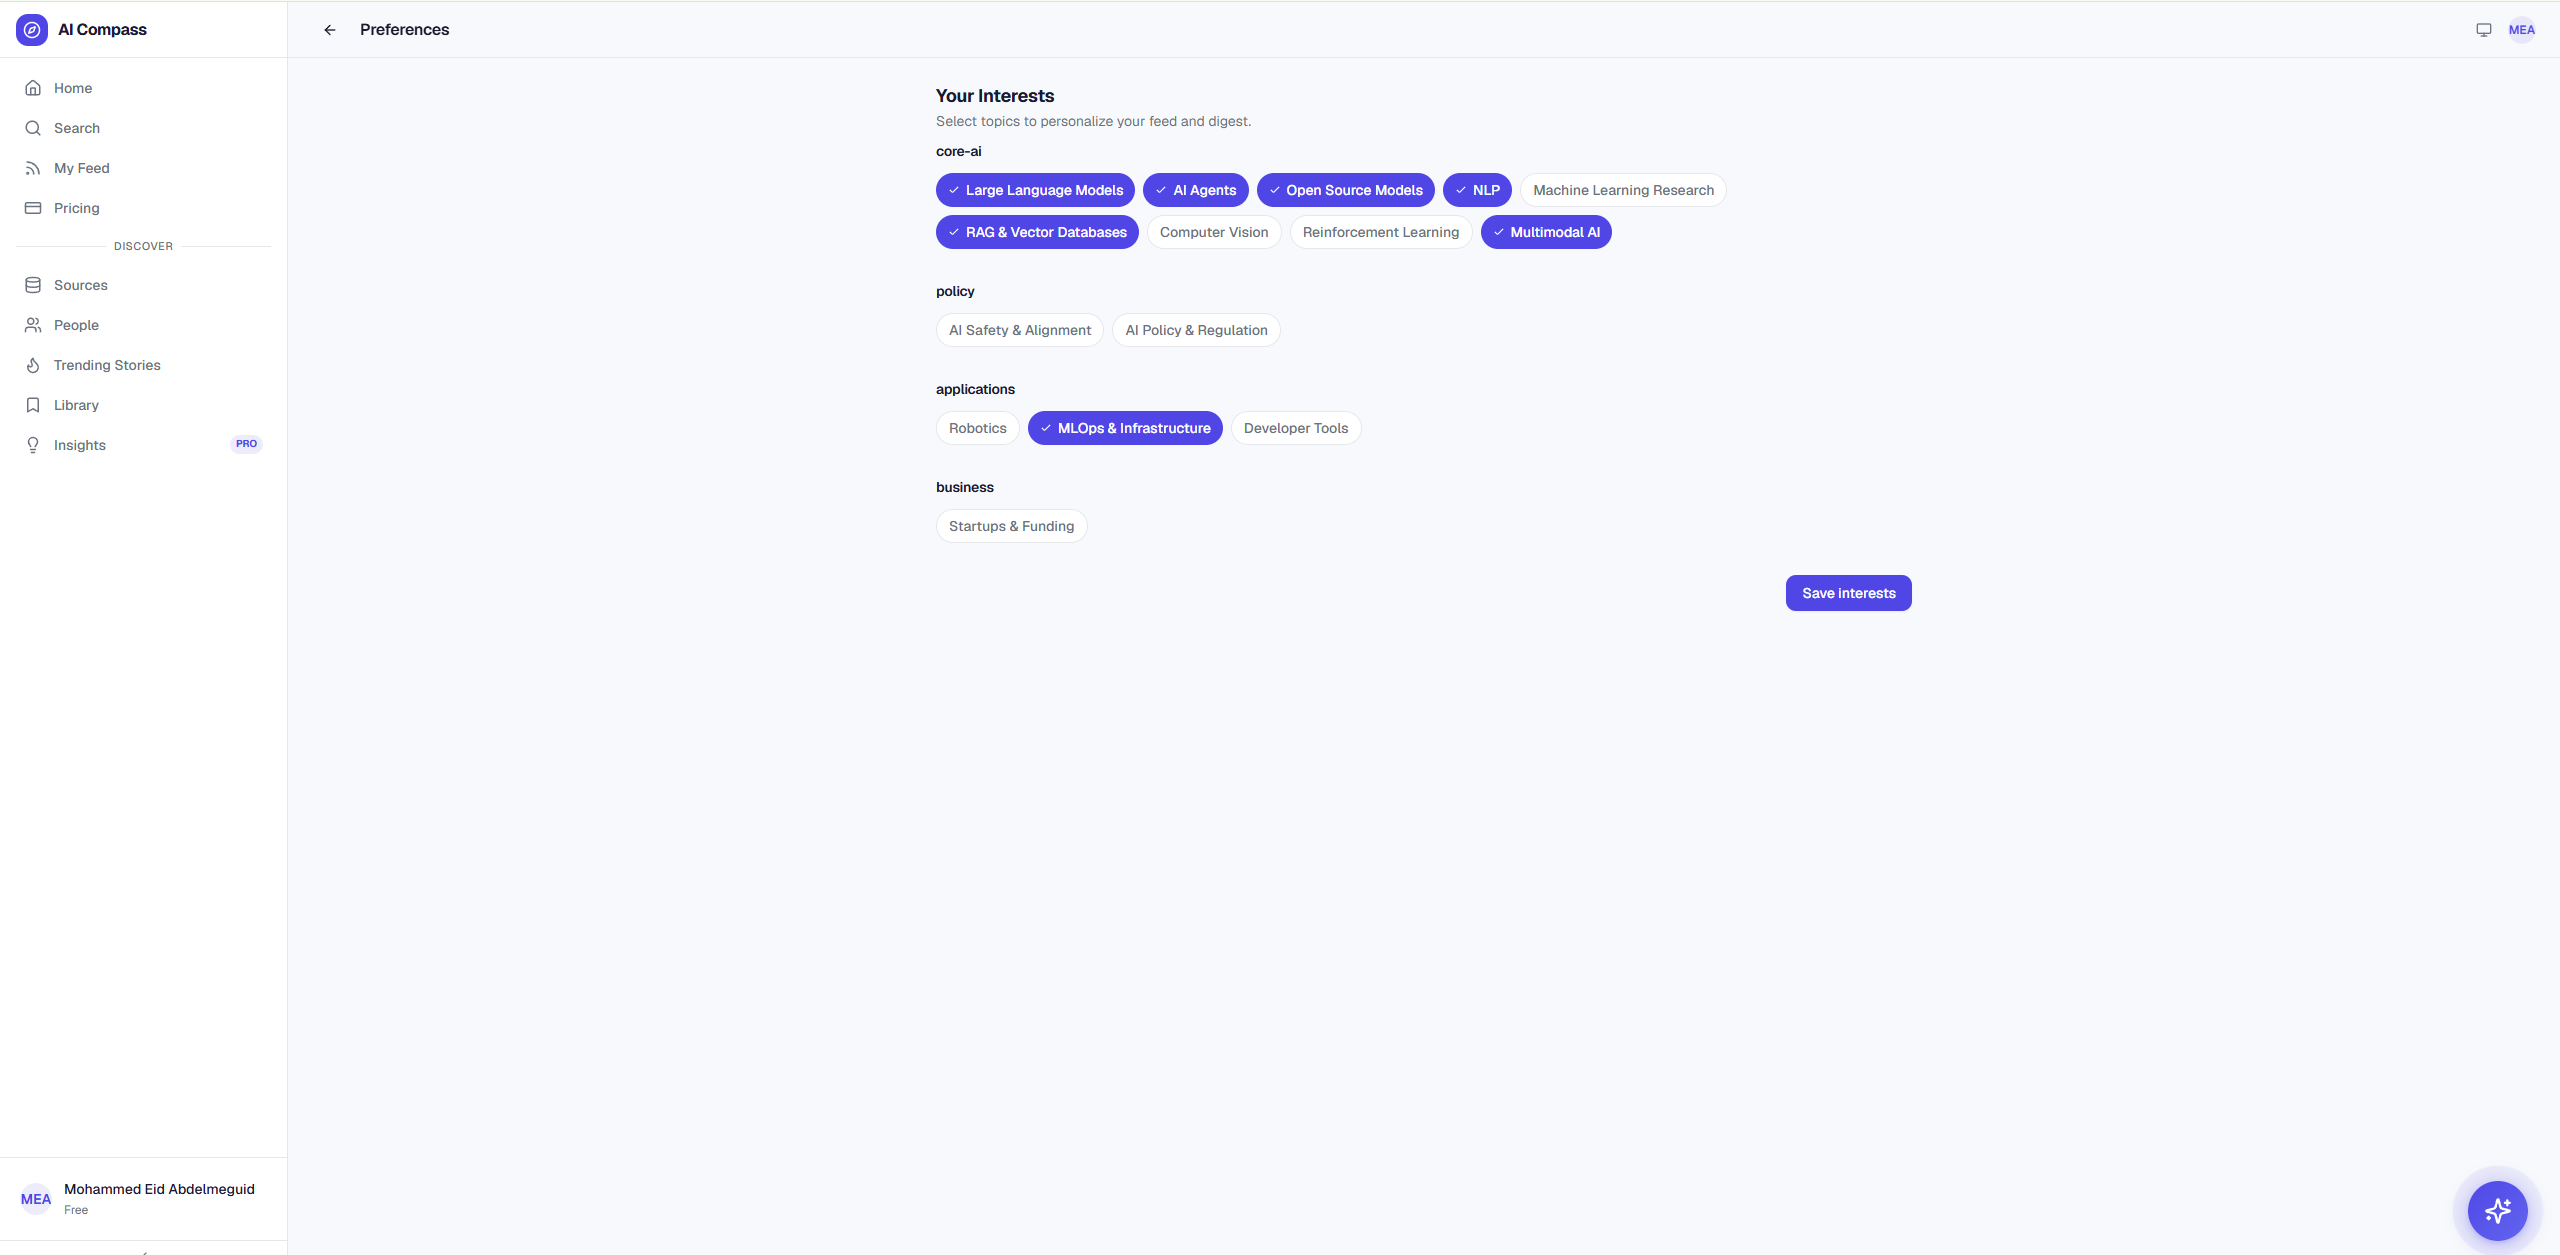
\includegraphics[width=0.85\textwidth]{figures/screenshots/screenshot_preferences.png}
\caption{The Preferences page, showing the interest-selection chip grid that seeds a new user's cold-start candidate generation (Leg B fallback, Section~\ref{sec:rec-candidates}).}
\label{fig:screenshot-preferences}
\end{figure}

\section{The Personalized Ranking Score}
\label{sec:rec-score}

Once a bounded candidate pool exists for a user, every candidate is scored by \texttt{RankingService.\_score()}. The score is built in three steps, expressed here as three equations, all implemented in the same function.

\begin{equation}
\text{base} = 0.35\,I + 0.20\,Q + 0.15\,F + 0.15\,S + 0.15\,N
\label{eq:ranking-base}
\end{equation}

\begin{itemize}
  \item $I$ (\emph{interest\_score}): the candidate's maximum per-topic \texttt{UserAffinity} weight (dimension \texttt{topic}), normalized by the user's own maximum topic-affinity weight, so that $I \in [0,1]$ regardless of how large or small a user's absolute affinity magnitudes are. If the user has no affinity data at all, a cold-start fallback applies: $I = 1.0$ if the item shares a topic with the interests the user selected during onboarding, and $I = 0.0$ otherwise.
  \item $Q$ (\emph{quality}): read directly from the \texttt{content\_scores.score} value, a separate quality heuristic computed once per item by the content-intelligence pipeline (Chapter~5) and never recomputed here; it defaults to $0.5$ if no score row yet exists for the item.
  \item $F$ (\emph{freshness}): $F = \exp\!\left(-\dfrac{\ln 2}{48}\cdot\text{age\_hours}\right)$, an exponential decay with a 48-hour half-life measured from the item's publication time to the present.
  \item $S$ (\emph{source\_affinity}): the item's per-source \texttt{UserAffinity} weight, normalized by the user's own maximum source-affinity weight in the same way as $I$; it defaults to $0.5$ if the user has no source-affinity data at all.
  \item $N$ (\emph{novelty}): $N = 1.0$ if the item has never been shown to this user, determined by a 30-day lookback over digest-email click tokens; otherwise $N = 1 - \exp\!\left(-\dfrac{\ln 2}{10}\cdot\text{age\_days}\right)$, a recovery curve with a 10-day half-life, where $\text{age\_days}$ is the time since the item was last shown. This is an important precision point: because ``shown'' is tracked exclusively through digest-email click tokens, $N$ in the current implementation measures ``has this item not recently been emailed to this user,'' not ``has this item not recently been viewed anywhere, including the web feed.'' A user who has already seen and read an item on the web feed, but never received it in a digest email, is still scored as though the item were fully novel, a real, disclosed precision gap rather than an intended design property, revisited in Section~\ref{sec:rec-limitations}.
\end{itemize}

The weighted sum in Equation~\ref{eq:ranking-base} is the largest single design decision AI Compass makes about what personalization means in this system: 35\% of the score rewards demonstrated topical interest, 20\% rewards independently assessed content quality, and the remaining 45\% is split evenly across recency, source loyalty, and novelty. These five weights are a project-specific configuration choice, not a value drawn from prior literature.

\begin{equation}
\text{final\_score} = \text{clamp}_{[0,1]}\Bigl(\text{base} \times M_{\text{depth}} \times M_{\text{format}} \times M_{\text{lean}} \times M_{\text{time}}\Bigr)
\label{eq:ranking-final}
\end{equation}

\begin{itemize}
  \item $M_{\text{depth}}$ compares the item's \texttt{content\_enrichment.technical\_depth} classification against the band implied by the user's stated expertise level.
  \item $M_{\text{format}}$ favors video or article content according to the user's stated format preference.
  \item $M_{\text{lean}}$ favors research-leaning or industry-leaning content according to the user's stated interest lean.
  \item $M_{\text{time}}$ penalizes content whose estimated reading or watch time exceeds the user's stated reading-time budget.
\end{itemize}

All four multipliers fall within roughly $[0.5, 1.15]$, and the codebase's own documentation is explicit that these are ``nudges, not hard filters'': no multiplier can ever drive a candidate's score to zero, only adjust it upward or downward by roughly 15--50\%. A candidate with strong base-signal support therefore always remains visible even if none of the four soft preferences line up with it, which is a deliberate property: the multipliers reflect stated stylistic preference, not a correctness gate on relevance.

\begin{equation}
\text{relevance\_score} = \text{clamp}\bigl(\text{round}(\text{final\_score} \times 10,\, 2),\, 0,\, 10\bigr)
\label{eq:ranking-relevance}
\end{equation}

Equation~\ref{eq:ranking-relevance} is purely presentational: it rescales the internal $[0,1]$ final score onto the more legible $[0,10]$ range (rounded to two decimal places) that is persisted to \texttt{user\_rankings} and, ultimately, shown wherever a relevance figure is surfaced to a user or an evaluator. Table~\ref{tab:ranking-signals} summarizes the five base-formula signals in one place.

\begin{table}[htbp]
\centering
\caption{The five weighted signals in the personalized ranking base score (Equation~\ref{eq:ranking-base}).}
\label{tab:ranking-signals}
\small
\begin{tabular}{|p{2.4cm}|p{1.3cm}|p{4.6cm}|p{4.8cm}|}
\hline
\textbf{Signal} & \textbf{Weight} & \textbf{Formula / Source} & \textbf{Notes} \\
\hline
Interest ($I$) & 0.35 & Max per-topic \texttt{UserAffinity}, normalized & Cold-start: 1.0/0.0 by onboarding topic overlap \\
\hline
Quality ($Q$) & 0.20 & \texttt{content\_scores.score} (Chapter~5) & Default 0.5 if no score row exists \\
\hline
Freshness ($F$) & 0.15 & $\exp(-\ln2/48 \times \text{age\_hours})$ & 48-hour half-life \\
\hline
Source affinity ($S$) & 0.15 & Max per-source \texttt{UserAffinity}, normalized & Default 0.5 if no data \\
\hline
Novelty ($N$) & 0.15 & $1$, or $1-\exp(-\ln2/10 \times \text{age\_days})$ & Measures ``not recently emailed,'' not ``not recently viewed'' \\
\hline
\end{tabular}
\end{table}

\section{Diversification: Maximal Marginal Relevance and Exploration}
\label{sec:rec-mmr}

A ranking that simply sorted candidates by \texttt{final\_score} would tend to repeatedly surface near-duplicates of whatever a user's affinities already favor, reinforcing rather than counteracting a filter bubble. AI Compass addresses this with Maximal Marginal Relevance (MMR), the established diversification method introduced by Carbonell and Goldstein~\cite{carbonell1998mmr}, applied here in its now-standard form: rather than picking items purely by relevance, MMR builds the output list greedily, at each step picking the candidate that best balances relevance against dissimilarity to what has already been selected.

\begin{equation}
\text{mmr\_score}(c) = \lambda \cdot \text{final\_score}(c) \;-\; (1-\lambda) \cdot \max_{s \,\in\, \text{selected}} \cos\bigl(\text{embed}(c), \text{embed}(s)\bigr)
\label{eq:mmr}
\end{equation}

Selection proceeds greedily: at each step, the remaining candidate with the highest $\text{mmr\_score}$ is appended to the selected list, and the process repeats until the output list's relevance quota is filled; ties are broken by earlier position in the candidate pool, a stable but not semantically meaningful tie-break rule. It is important to distinguish two different things in Equation~\ref{eq:mmr}: MMR itself, the general subtraction of a similarity-to-already-selected penalty from a relevance term, is the established method from the information-retrieval literature~\cite{carbonell1998mmr}, while the specific value $\lambda = 0.7$ is an AI Compass project-specific configuration choice, not a value drawn from Carbonell and Goldstein's paper or from any other source; it simply reflects this project's own judgement that relevance should dominate diversity roughly 70/30 in the trade-off.

Separately from MMR, AI Compass reserves a fixed fraction of the output list's slots for a distinct, deliberate filter-bubble countermeasure: an \emph{exploration slice}. When the output list has at least five total slots, approximately 12\% of them are filled not by MMR selection but by a weighted-random draw over the leftover candidates, the ones MMR did not select. Each leftover candidate's draw weight is its own \texttt{final\_score}, floored at 0.01 so that no candidate has literally zero chance of being drawn. This weighting is a deliberate middle ground: it is biased toward candidates that scored reasonably but not at the very top, rather than being either pure noise (a uniform draw over everything) or a disguised extension of the same top-relevance ordering MMR already produces.

This mechanism carries one limitation that should be stated plainly rather than left implicit: the weighted draw is implemented with Python's unseeded \texttt{random.random()}, which means the exploration slice for a given user and candidate pool is genuinely \emph{not} reproducible from one ranking run to the next. Two ranking passes over an identical candidate pool for the same user can select different items for the exploration slots purely due to this randomness. This is a disclosed, real property of the current implementation, not a design intention; a reproducible variant would seed the draw deterministically per user and per ranking run, and this is noted again as a limitation in Section~\ref{sec:rec-limitations}.

\section{Explanation Generation}
\label{sec:rec-explanations}

Every item that survives selection is paired with an explanation of why it was chosen, and this explanation is generated by pure string templating; there is no large language model call anywhere on this path. \texttt{RankingService}'s explanation builder inspects which of a small set of conditions hold for the selected item (a matched topic, a followed-entity or followed-source match, unusually high source affinity, unusually high freshness, unusually high quality) and composes whichever clauses apply into a single sentence beginning ``Recommended because\ldots''. Items filled by the exploration slice (Section~\ref{sec:rec-mmr}) receive a fixed, separate explanation string instead: ``A change of pace from your usual topics, worth a look.'' This is not a templated composition of matched signals, since by construction those items were not chosen for scoring an unusually good match.

This design is worth calling out as a clean, positive confirmation of one of the project's own stated goals: a fully explainable, non-generative ranking pipeline. Every explanation shown to a user is fully deterministic given the same scored item and the same set of matched conditions, is computed with negligible latency and cost relative to a generative call, and is traceable directly back to the specific signal or signals that produced it; there is no possibility of an explanation inventing a reason that does not correspond to an actual computed signal, because the templating logic can only ever select from the fixed set of clauses it was given.

\section{The Public (Non-Personalized) Home Feed}
\label{sec:rec-public-feed}

A visitor who is not logged in still sees an ordered Home feed, but it is produced by an entirely separate, considerably simpler formula, implemented in \texttt{web/apps/news/feed\_ranking.py} rather than in \texttt{RankingService}:

\begin{equation}
\text{score} = 0.65\,F_{\text{page}} + 0.35\,Q - \text{penalty}
\label{eq:public-feed}
\end{equation}

Here $Q$ is the same content-quality value used elsewhere, but $F_{\text{page}}$ is deliberately \emph{not} the same freshness computation as Equation~\ref{eq:ranking-base}'s $F$: it is measured relative to the newest item appearing on the current page being rendered, rather than relative to wall-clock ``now.'' The penalty term is an anti-repetition mechanism unrelated to personalization: it adds 0.08 for every prior pick in the same list that came from the same source, plus a further 0.18 once a single source has produced two or more picks in a row, so that a source with an unusually large volume of recent content cannot dominate consecutive positions in the public feed. This formula is computed inline, freshly, for every HTTP request that renders the public Home feed; it is never persisted to any table and never varies by user, because there is no user-specific state to vary it by. It must not be read as a simplified or degraded version of the personalized ranker described in Section~\ref{sec:rec-score}; the two share no code, no weights, and no behavioral signal, and exist to solve genuinely different problems.

\section{Pipeline Summary}
\label{sec:rec-pipeline}

\begin{figure}[htbp]
\centering
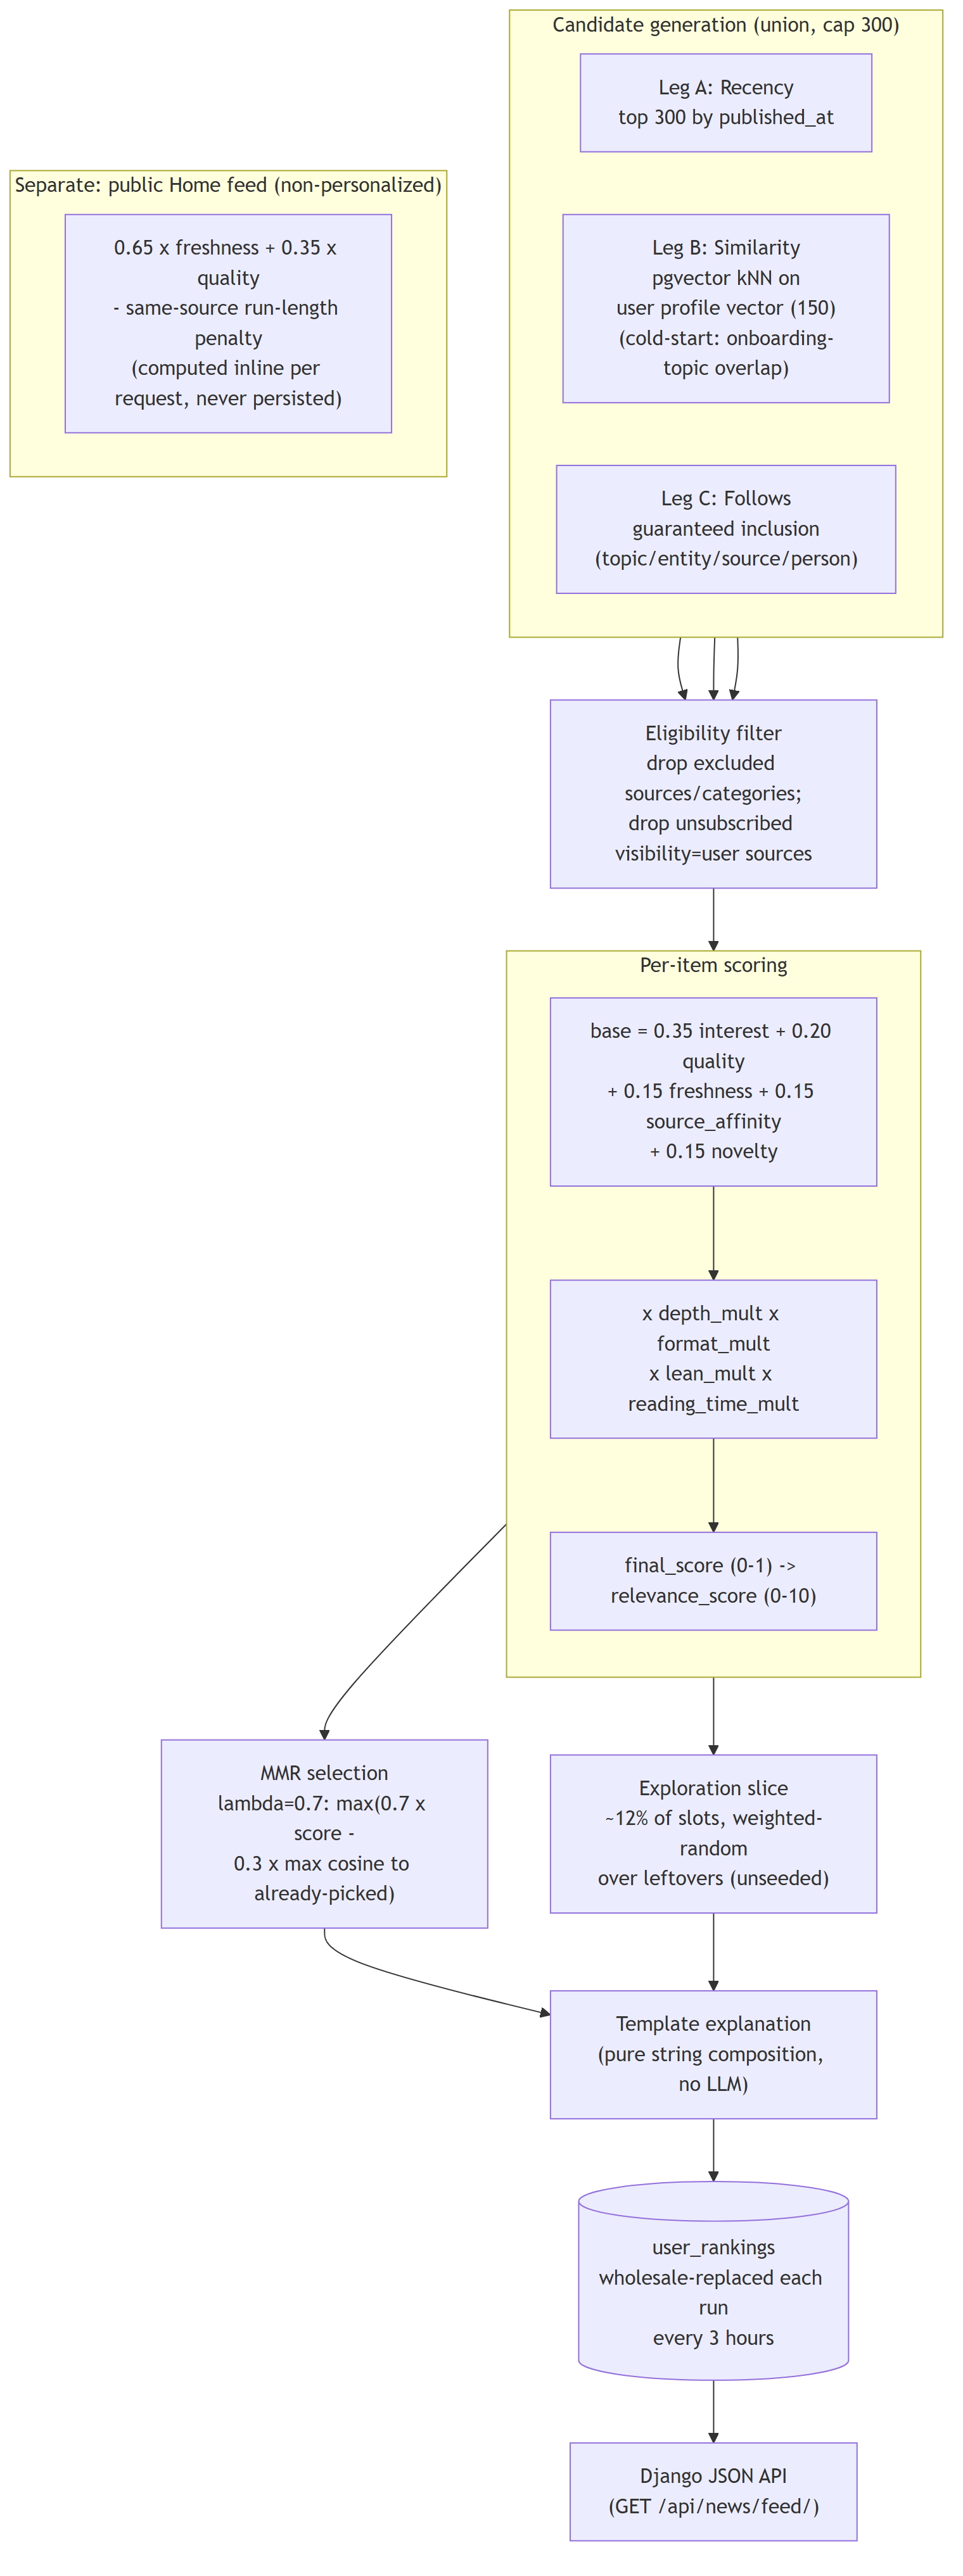
\includegraphics[width=0.55\textwidth,height=0.88\textheight,keepaspectratio]{figures/ranking_pipeline.png}
\caption{The personalized ranking pipeline: three-leg candidate generation, eligibility filtering, weighted-signal scoring, MMR diversification with a reserved exploration slice, and templated explanation generation.}
\label{fig:ranking-pipeline}
\end{figure}

Figure~\ref{fig:ranking-pipeline} lays out the personalized pipeline end to end. A feed request first applies the eligibility filter (Section~\ref{sec:rec-candidates}), then the surviving pool feeds the three-leg candidate union capped at 300 (Algorithm~\ref{alg:candidates}). Every candidate is scored deterministically through Equations~\ref{eq:ranking-base}--\ref{eq:ranking-relevance}, drawing on the nightly decayed affinities and profile vector (Equation~\ref{eq:affinity-decay}). Scored candidates pass through MMR selection (Equation~\ref{eq:mmr}), which fills most slots under the relevance/diversity trade-off, while a reserved exploration slice fills the remaining $\approx$12\% via a weighted random draw over MMR's leftovers. Every selected item, MMR-chosen or exploration-chosen, is paired with a templated explanation before persistence to \texttt{user\_rankings}. No stage calls a large language model.

Figure~\ref{fig:screenshot-myfeed} shows My Feed, the page this pipeline ultimately renders into for a signed-in user: each card is prefixed with the templated explanation string described in Section~\ref{sec:rec-explanations} (for example, ``Recommended because it published recently'' or ``Recommended because it from a source you engage with often, and published recently''), making the connection between the scoring pipeline and what the user actually sees directly visible rather than left to the reader's imagination.

\begin{figure}[htbp]
\centering
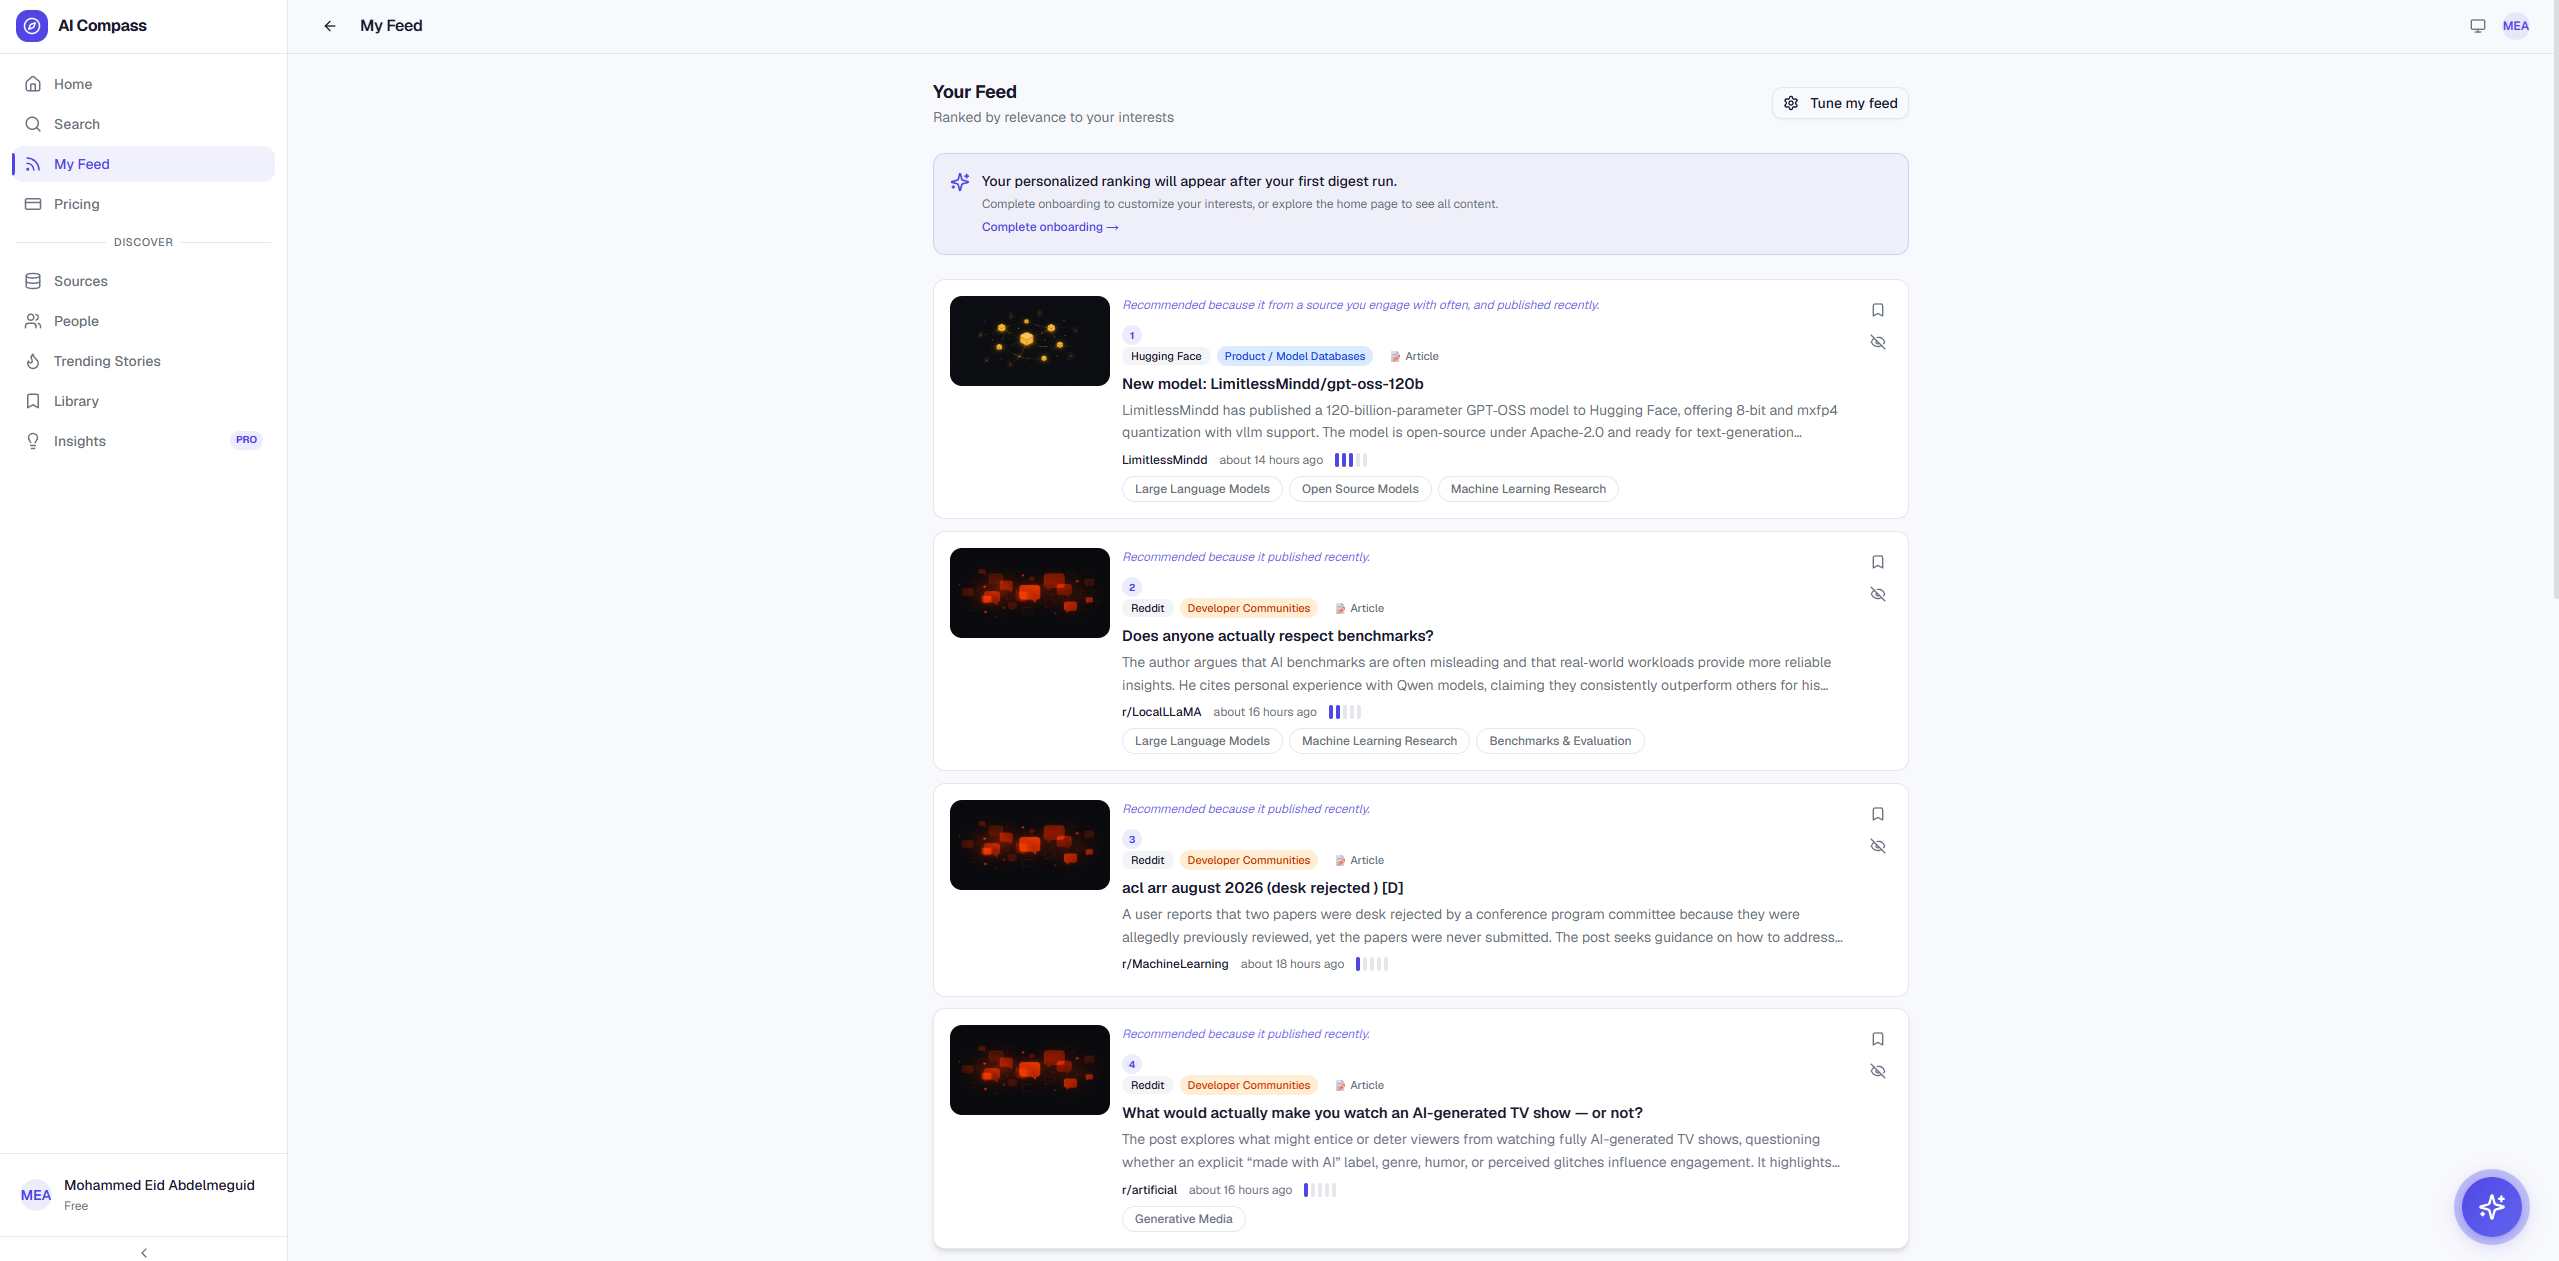
\includegraphics[width=0.85\textwidth]{figures/screenshots/screenshot_myfeed.png}
\caption{My Feed, showing the per-item templated explanation strings (Section~\ref{sec:rec-explanations}) that accompany each ranked recommendation.}
\label{fig:screenshot-myfeed}
\end{figure}

\section{Deliberately Deferred Approaches}
\label{sec:rec-deferred}

Several more sophisticated approaches were considered and explicitly left out of scope, rather than overlooked:

\begin{itemize}
  \item \textbf{Neural or learned ranking}: deferred; it would need substantially more logged interaction data than currently exists to train or validate, the same data-scarcity finding Chapter~10 documents directly.
  \item \textbf{Collaborative filtering}: deferred; the classic cold-start problem at a small user base leaves too little cross-user co-engagement signal to outperform the content-based approach already in place.
  \item \textbf{Per-persona summaries}: deferred to keep the one-LLM-call-per-item enrichment budget growing per-item, not per-user.
  \item \textbf{Region and language filters}: deferred; the current content pool and user base are not yet large or linguistically diverse enough for such filters to be meaningful.
  \item \textbf{Manual per-source weight sliders}: deferred in favor of the existing follow/exclude and source-affinity mechanisms, which already cover most of the same use case with less interface complexity.
  \item \textbf{Audience tags} (beyond the existing \texttt{technical\_depth} field): deferred as an enrichment dimension not yet justified by a concrete downstream use.
\end{itemize}

\section{Known Limitations of the Current Formula}
\label{sec:rec-limitations}

Three real, disclosed gaps are worth restating together, plainly, rather than left scattered.

First, \texttt{UserAffinity} maintains three dimensions (\texttt{topic}, \texttt{source}, \texttt{entity}), and entity-level affinity \emph{is} computed nightly (Section~\ref{sec:rec-signals}), but Equation~\ref{eq:ranking-base} only ever reads \texttt{topic} and \texttt{source} for $I$ and $S$; \texttt{entity} is computed but never consumed. This is a genuine, unaddressed gap, not a deliberate decision; the dimension exists specifically to feed personalization, and currently does not.

Second, the novelty signal $N$ (Section~\ref{sec:rec-score}) is tracked exclusively through digest-email click tokens, so it really measures ``not recently emailed,'' not ``not recently viewed on the web feed.'' A user who reads an item on the web but never receives it by email is scored as though it were fully novel indefinitely.

Third, the exploration slice's weighted draw (Section~\ref{sec:rec-mmr}) uses Python's unseeded \texttt{random.random()}, so exploration-slot items are not reproducible across repeated runs over an identical pool; the deterministic MMR-selected majority is unaffected, but the exploration slice cannot be replayed exactly without a seeded source.

None of these three gaps invalidate the ranker's core determinism claim for the MMR-selected portion of the list, and none were hidden in the implementation; all three are visible directly in the code and, in the case of the entity-affinity gap, in the mismatch between what is computed nightly and what the scoring function actually reads. They are recorded here, and again in Chapter~11, as concrete, well-scoped items for future work rather than as an indictment of the current design.
